\documentclass[border=10pt]{standalone}

\usepackage{tikz}
\usepackage{tikzsymbols}
\usetikzlibrary{calc,patterns,shapes.geometric}

\def\centerarc[#1](#2)(#3:#4:#5){\draw[#1] ($(#2)+({#5*cos(#3)},{#5*sin(#3)})$) arc (#3:#4:#5);}

\begin{document}
	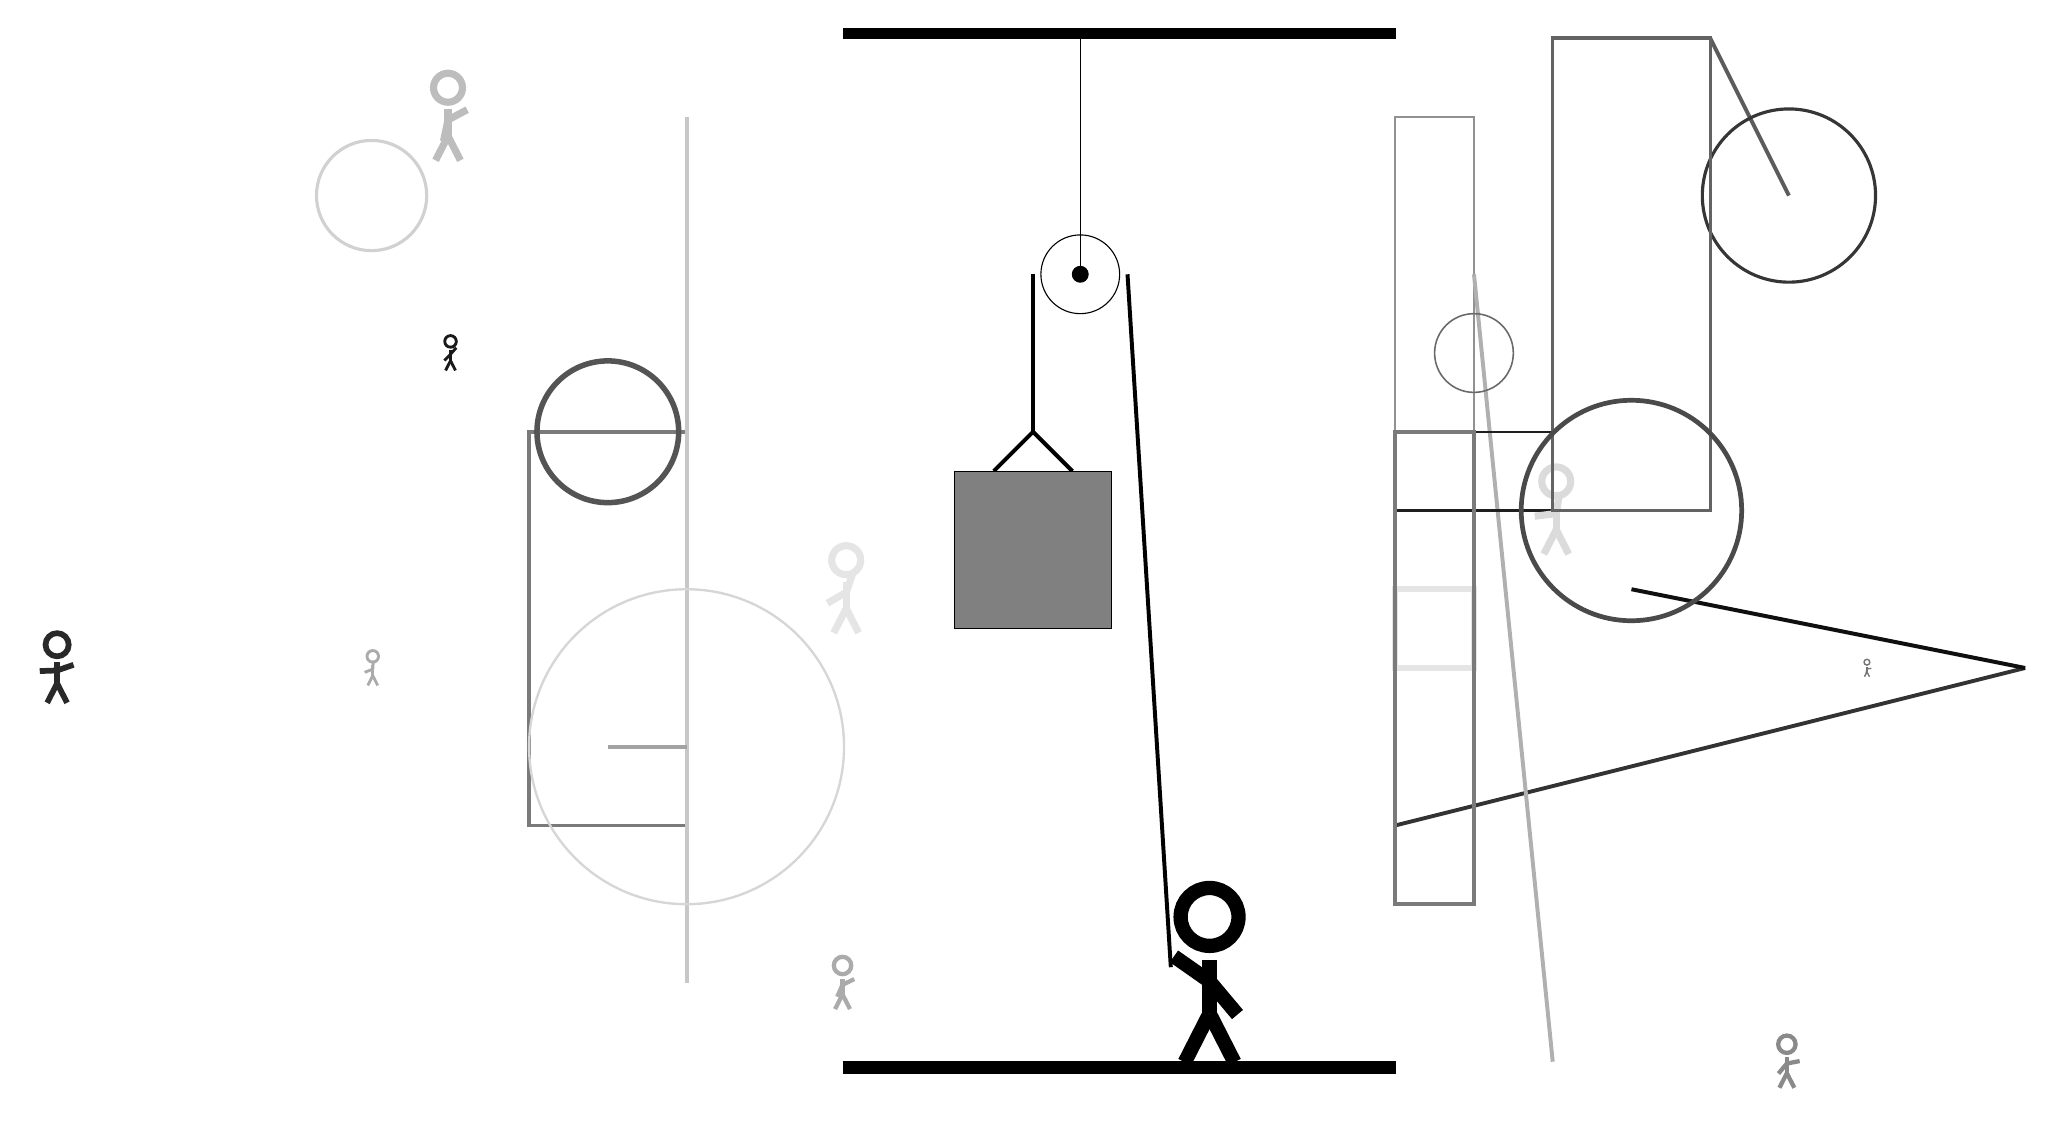
\begin{tikzpicture}
		%%%%% START %%%%%
		
		\draw[fill=black] (-2, 10) rectangle (5, 10.125);
		
		\draw[line width=0.5mm, color=black!80](5, 0) -- (13, 2);
		
		\node[line width=0.4mm, color=black!46] at (10, -3) {\Strichmaxerl[3][50][11]};
		\draw[line width=0.7mm, color=black!10] (6, 2) rectangle (5, 3);
		\draw[line width=0.2mm, color=black!43] (5, 5) rectangle (6, 9);
		\draw[line width=0.5mm, color=black!64](9, 10) -- (10, 8);
		
		\node[line width=0.6mm, color=black!33] at (-2, -2) {\Strichmaxerl[3][66][26]};
		
		\draw [line width=0.4mm, color=black!18](-8, 8) circle (0.7);
		
		\node[line width=0.4mm, color=black!84] at (-12, 2) {\Strichmaxerl[4][2][19]};
		\draw[line width=0.5mm, color=black!52] (-4, 5) rectangle (-6, 0);
		\draw[line width=0.5mm, color=black!31](6, 7) -- (7, -3);
		
		\draw[line width=0.5mm, color=black!22](-4, -2) -- (-4, 9);
		\draw[line width=0.3mm, color=black!88] (5, 4) rectangle (7, 5);
		\draw[line width=0.5mm, color=black!52] (5, 5) rectangle (6, -1);
		
		\node[line width=0.7mm, color=black!10] at (-2, 3) {\Strichmaxerl[5][30][71]};
		\node[line width=0.4mm, color=black!14] at (7, 4) {\Strichmaxerl[5][7][81]};
		\node[line width=0.7mm, color=black!33] at (-8, 2) {\Strichmaxerl[2][21][86]};
		
		\draw [line width=0.3mm, color=black!16](-4, 1) circle (2.0);
		
		\draw [line width=0.4mm, color=black!79](10, 8) circle (1.1);
		\draw[line width=0.5mm, color=black!36](-4, 1) -- (-5, 1);
		
		\node[line width=0.4mm, color=black!90] at (-7, 6) {\Strichmaxerl[2][45][49]};
		\node[line width=0.5mm, color=black!26] at (-7, 9) {\Strichmaxerl[5][78][28]};
		
		\draw [line width=0.7mm, color=black!67](-5, 5) circle (0.9);
		
		\draw [line width=0.2mm, color=black!59](6, 6) circle (0.5);
		\draw[line width=0.4mm, color=black!61] (7, 4) rectangle (9, 10);
		\node[line width=0.5mm, color=black!54] at (11, 2) {\Strichmaxerl[1][81][2]};
		
		\draw[line width=0.5mm, color=black!94](8, 3) -- (13, 2);
		\draw [line width=0.6mm, color=black!71](8, 4) circle (1.4);
		
		\draw (1, 7) circle (0.5);
		\draw[fill=black] (1, 7) circle (0.1);
		\draw (1, 10) -- (1, 7);
		
		\draw[line width=0.5mm] (-0.1, 4.5) -- (0.4, 5.0) -- (0.9, 4.5);
		\draw[fill=black!50] (-0.6, 4.5) rectangle (1.4, 2.5);
		
		\draw[line width=0.5mm] (0.4, 7) -- (0.4, 5.0);
		\centerarc[line width=0.5mm](1, 7)(0:180:0.6);
		\draw[line width=0.5mm](1.6, 7) -- (2.15, -1.8);
		
		\node at (2.6, -1.9) {\Strichmaxerl[10][-35][-50]};
		
		\draw[fill=black] (-2, -3) rectangle (5, -3.15);
		
		%%%%% END %%%%%
	\end{tikzpicture}
\end{document}